\enlargethispage{2.0\baselineskip}
\section*{\phantom{a}\hfill{}Scoring Summary\hfill\phantom{a}}

\medskip

\begin{minipage}{1.5cm}
\tikz{\node[draw, thick, minimum width=1.5cm, minimum height=1.5cm, inner sep=0pt, rounded corners=3mm] at (0,0) {
\includegraphics[width=1.0cm]{Images/gold-coins.png}};}
\end{minipage}
\ 
\begin{minipage}{6cm}
\raggedright
\textbf{Stack of Gold Coins (11):}\goldtext
\end{minipage}

\begin{minipage}{1.5cm}
\tikz{\node[draw, thick, minimum width=1.5cm, minimum height=1.5cm, inner sep=0pt, rounded corners=3mm] at (0,0) {
\includegraphics[height=1.25cm]{Images/bottle-of-rum.png}};}
\end{minipage}
\ 
\begin{minipage}{6cm}
\raggedright
\textbf{Bottle of Rum (9):} Score points based on how many bottles of rum you have at the end of the game. 0:0, 1:1, 2:4, 3:9, 4+:0.
\end{minipage}

\begin{minipage}{1.5cm}
\tikz{\node[draw, thick, minimum width=1.5cm, minimum height=1.5cm, inner sep=0pt, rounded corners=3mm] at (0,0) {
\includegraphics[height=1.0cm]{Images/black-spot-small.png}};}
\end{minipage}
\ 
\begin{minipage}{5.75cm}
\raggedright
\textbf{The Black Spot (1):} After each round, steal one random treasure from another character. Lose five points if you have the black spot at~the end of the game.
\end{minipage}

\begin{minipage}{1.5cm}
\tikz{\node[draw, thick, minimum width=1.5cm, minimum height=1.5cm, inner sep=0pt, rounded corners=3mm] at (0,0) {
\includegraphics[width=1.0cm]{Images/emerald.png}};}
\end{minipage}
\ 
\begin{minipage}{6cm}
\raggedright
\textbf{Emerald (7):}\emeraldtext
\end{minipage}

\begin{minipage}{1.5cm}
\tikz{\node[draw, thick, minimum width=1.5cm, minimum height=1.5cm, inner sep=0pt, rounded corners=3mm] at (0,0) {
\includegraphics[height=1.25cm]{Images/sapphire.png}};}
\end{minipage}
\ 
\begin{minipage}{6cm}
\raggedright
\textbf{Sapphire (7):}\sapphiretext
\end{minipage}

\begin{minipage}{1.5cm}
\tikz{\node[draw, thick, minimum width=1.5cm, minimum height=1.5cm, inner sep=0pt, rounded corners=3mm] at (0,0) {
\includegraphics[width=1.0cm]{Images/ruby.png}};}
\end{minipage}
\ 
\begin{minipage}{6cm}
\raggedright
\textbf{Ruby (7):}\rubytext
\end{minipage}

\newpage
\enlargethispage{2.0\baselineskip}
\section*{\phantom{a}\hfill{}Scoring Summary\hfill\phantom{a}}

\medskip


\begin{minipage}{1.5cm}
\tikz{\node[draw, thick, minimum width=1.5cm, minimum height=1.5cm, inner sep=0pt, rounded corners=3mm] at (0,0) {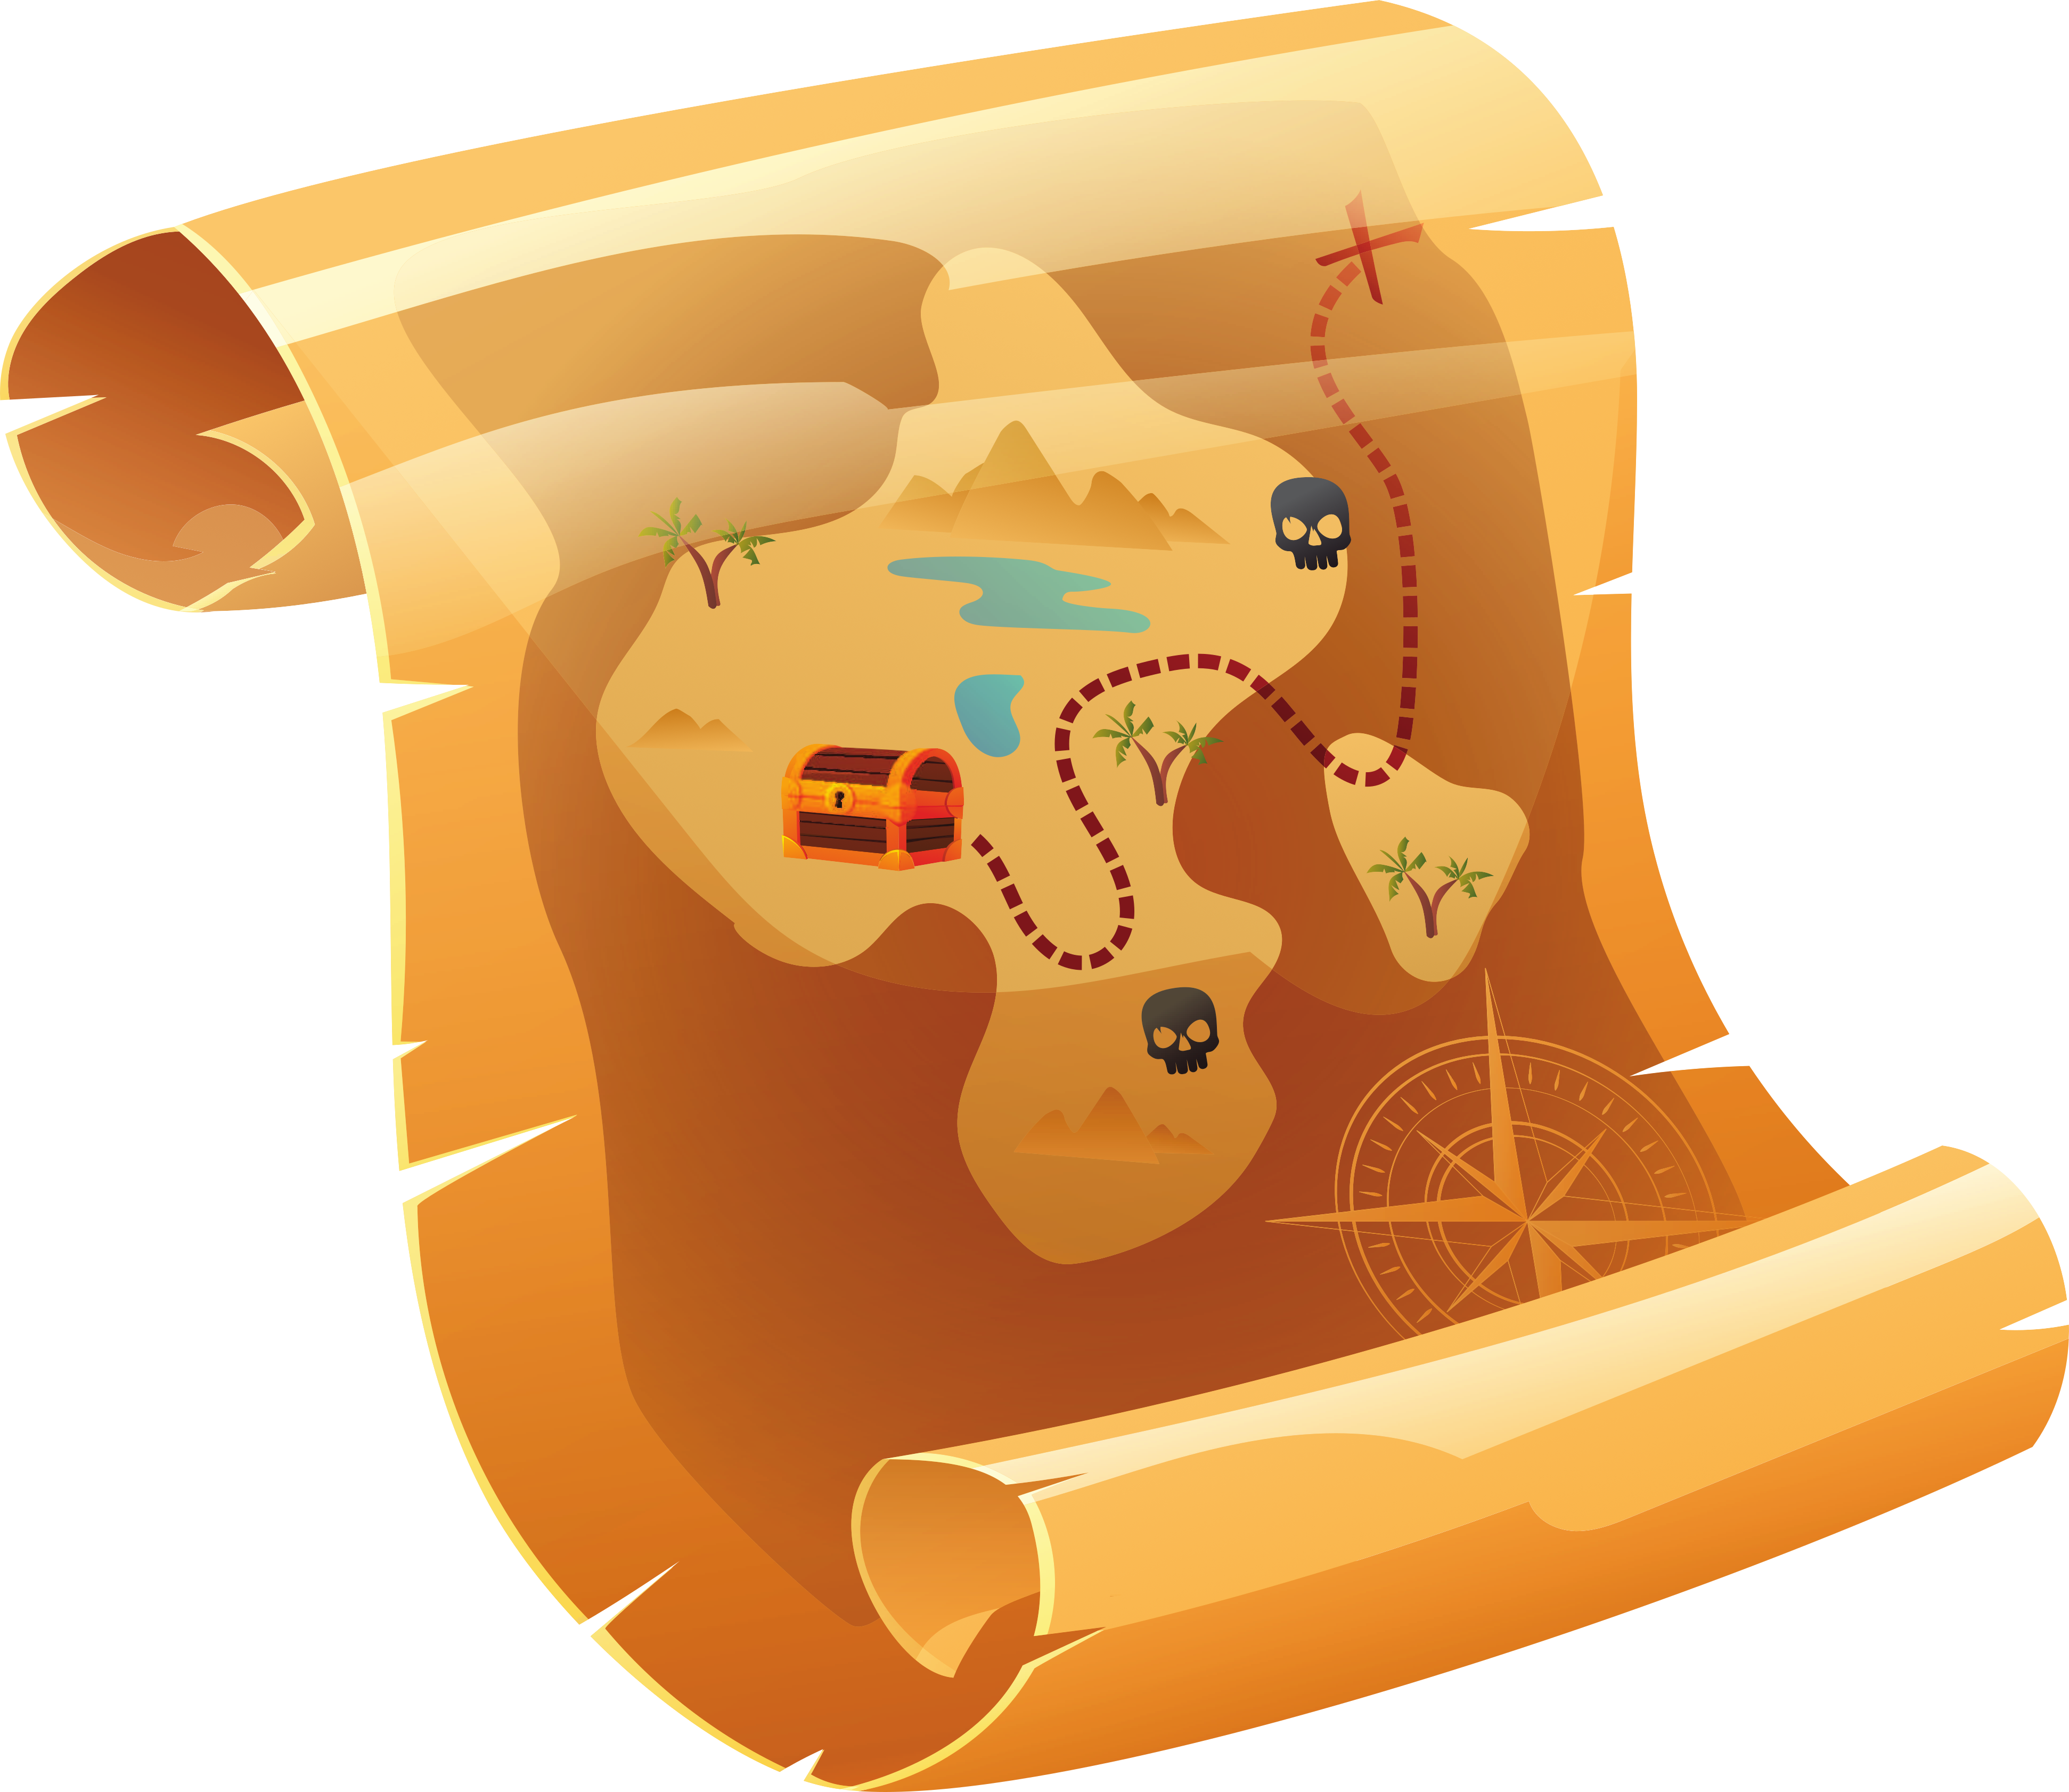
\includegraphics[width=1.0cm]{Images/treasure-map.png}};}
\end{minipage}
\ 
\begin{minipage}{6cm}
\raggedright
\textbf{Treasure Map (3):} \maptext
\end{minipage}

\begin{minipage}{1.5cm}
\tikz{\node[draw, thick, minimum width=1.5cm, minimum height=1.5cm, inner sep=0pt, rounded corners=3mm] at (0,0) {
\includegraphics[height=1.0cm]{Images/compass.png}};}
\end{minipage}
\ 
\begin{minipage}{6cm}
\raggedright
\textbf{Compass (2):}\compasstext
\end{minipage}

\begin{minipage}{1.5cm}
\tikz{\node[draw, thick, minimum width=1.5cm, minimum height=1.5cm, inner sep=0pt, rounded corners=3mm] at (0,0) {
\includegraphics[height=1.0cm]{Images/spyglass.png}};}
\end{minipage}
\ 
\begin{minipage}{6cm}
\raggedright
\textbf{Spyglass (2):}\spyglasstext
\end{minipage}

\begin{minipage}{1.5cm}
\tikz{\node[draw, thick, minimum width=1.5cm, minimum height=1.5cm, inner sep=0pt, rounded corners=3mm] at (0,0) {
\includegraphics[height=1.0cm]{Images/message-in-a-bottle.png}};}
\end{minipage}
\ 
\begin{minipage}{6cm}
\raggedright
\textbf{Message in a Bottle (2):}\messagetext
\end{minipage}

\begin{minipage}{1.5cm}
\tikz{\node[draw, thick, minimum width=1.5cm, minimum height=1.5cm, inner sep=0pt, rounded corners=3mm] at (0,0) {
\includegraphics[width=1.0cm]{Images/pistol.png}};}
\end{minipage}
\ 
\begin{minipage}{5.5cm}
\raggedright
\textbf{Pistol (6):} You may discard a pistol at any time to steal one treasure from another character.
\end{minipage}

\begin{minipage}{1.5cm}
\tikz{\node[draw, thick, minimum width=1.5cm, minimum height=1.5cm, inner sep=0pt, rounded corners=3mm] at (0,0) {
\includegraphics[height=1.0cm]{Images/barrel.png}};}
\end{minipage}
\ 
\begin{minipage}{6cm}
\raggedright
\textbf{Barrel (5):} You may discard a barrel at any time to draw a random secret treasure card. 
\end{minipage}
